Con riferimento alla matrice $A_\mathrm{N}$ definita in (1), risolvere il sistema lineare $$A_\mathrm{N}\textbf{x} = \begin{pmatrix}1 \\ \vdots \\ 1\end{pmatrix} \in\mathbb{R}^{N}, $$
con i metodi di Jacobi e Gauss-Seidel, per $N = 10 : 10 : 500$, partendo dalla approssimazione nulla della soluzione, ed imponendo che la norma del residuo sia minore di $10^{-8}$. Utilizzare, a tal fine, la function dell'esercizio 26, scrivendo function ausiliarie \textit{ad hoc} (vedi esercizio 27) che sfruttino convenientemente la struttura di sparsità (nota) della matrice $A_\mathrm{N}$. Graficare il numero delle iterazioni richieste dai due metodi iterativi, rispetto ad $N$, per soddisfare il criterio di arresto prefissato.
\hspace*{\fill}
\par\noindent\rule{\textwidth}{0.4pt}
\hspace*{\fill}

\textbf{Prodotto \textit{ad hoc} matrice vettore}:
\lstinputlisting[language=Matlab]{Chapter-6/Exercise-28/matvec.m}
\textbf{Metodo di Jacobi}:
\lstinputlisting[language=Matlab]{Chapter-6/Exercise-28/jacobi.m}
\textbf{Metodo di Gauss-Seidel}:
\lstinputlisting[language=Matlab]{Chapter-6/Exercise-28/gs.m}
\begin{lstlisting}[language=Matlab, caption=Codice Matlab]
x = linspace(10, 500, 50);
tol = 1E - 8;
ij = zeros(50, 1);
igs = zeros(50, 1);
for n = 10 : 10 : 500
    b = ones(n, 1);
    x0 = zeros(n, 1);
    [x, i] = splitting(b, @matvec, @jacobi, x0, tol);
    ij(n / 10) = i;
    [x, i] = splitting(b, @matvec, @gs, x0, tol);
    igs(n / 10) = i;
end
plot(x, ij, x, igs);
legend('Jacobi', 'Gauss-Seidel');
\end{lstlisting}
La seguente figura mostra il confronto del numero di iterazioni necessarie ai metodi di \textit{Jacobi} e \textit{Gauss-Seidel}, al variare della dimensione della matrice  $A_\mathrm{N}$ con $N = 10 : 10 : 500$:
\begin{figure}[H]
	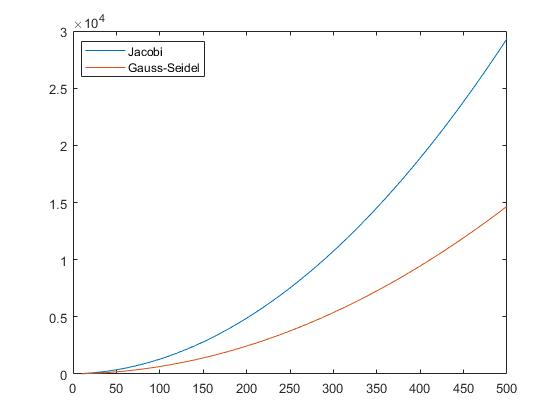
\includegraphics[width=\textwidth]{Chapter-6/Exercise-28/plot.jpg}
	\caption*{Numero iterazioni dei metodi di \textit{Jacobi} e \textit{Gauss-Seidel} con $N = 10 : 10 : 500$}
\end{figure}
